\chapter{Plataforma de desarrollo}
\label{cap:capitulo4}
\setcounter{footnote}{16}
 
Con los objetivos del proyecto definidos, en este capítulo se abordarán las distintas plataformas de desarrollo, tanto \textit{hardware} como \textit{software}, que han facilitado el logro de esos objetivos.

\section{Hardware}
\label{sec:hardware}

Este apartado recoge la descripción de los componentes \textit{hardware} utilizados en este proyecto, para los cuales se ha buscado priorizar la reducción de costes en cada elección y utilizar aquellos elementos a los que se tenía acceso a la hora del desarrollo del proyecto o de los que se disponía a la hora de elaborarlo.

\subsection{Cámara Logitech C270 HD}
\label{subsec:logiC270HD}

Esta cámara web (Figura \ref{fig:logiC270HD}) de dimensiones 72,91 x 31,91 x 66,64 mm, corrige la iluminación de manera automática, produciendo colores reales y naturales y ajustándose a las condiciones de iluminación del entorno, lo que facilita la detección de fresas. Ofrece una resolución HD 720p, proporcionando imágenes claras y nítidas a una velocidad de 30 fotogramas por segundo (fps) con una lente que cuenta con enfoque fijo y un campo visual diagonal (dFoV) de 55 grados. Su coste aproximado es, en la página oficial, de 44€, aunque en otras empresas destacadas en el sector de la electrónica y la tecnología en España puede encontrarse por, aproximadamente, 25€.

\begin{figure} [h!]
    \begin{center}
      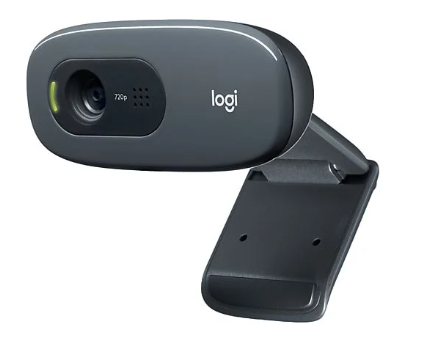
\includegraphics[width=7cm]{figs/logi C270.png}
    \end{center}
    \caption{Cámara Logitech C270 HD$^{\ref{note:enlace16}}$}
    \label{fig:logiC270HD}
\end{figure}


\footnotetext[\value{footnote}]{\url{https://www.logitech.com/es-es/products/webcams/c270-hd-webcam.960-001063.html?srsltid=AfmBOor4HptUTcGrxE-4SZxKR-ARw-ykNeagHSEzXUvTlXkx8qLfY4lG}\label{note:enlace16}}


\subsection{Soporte de brazo articulado}
\label{subsec:soporte}

Para poder ubicar la cámara en una posición fija que permita 

\subsection{Ordenador principal}
\label{subsec:ordenador}

\subsection{Robot de Universal Robots de la gama e-series}
\label{subsec:URe-series}

\section{Software}
\label{sec:software}

\subsection{Ubuntu}
\label{sec:ubuntu}

\subsection{Python}
\label{sec:python}

\subsection{OpenCV}
\label{sec:OpenCV}

\subsection{Anaconda}
\label{sec:Anaconda}

\subsection{YOLOv3}
\label{sec:YOLOv3}

\subsection{PyTorch}
\label{sec:PyTorch}


